%\section{Protocol ARM implementation}
\label{sec:armspi}
One integral part of the project is the communication between the microprocessor and FPGA. This section describes the process of implementing SPI communication software, for the remainder of this section just referred to as the \textit{implementation}, on the microprocessor. It will go over the initial demands of the implementation, how it was made, how it works, and how it is supposed to be used by other parts of the system. A test of the implementation is also described. Finally, the results the test yielded, plus thoughts about further improvements, are discussed.

\subsection{Requirements and delimitations}\label{sec:spi_software_reqs}
The first part of the development process was to specify requirements to the implementation, to make it easier for the rest of the software system to make use of the SPI link. Those requirements were:
\begin{enumerate}
  \item The implementation would have to be multi-task- and thread safe, as more than one task may have to use the SPI software interface at any given time.
  \item The interface provided by the implementation should be easy to use by other processes in the system.
\end{enumerate}

To fulfill the first requirement, some problems has to be considered carefully: If more than one task uses the implementations interface to send data asynchronously, how do they receive data back in the correct order? There is only one physical SPI link in the LM3S6965, so it has to be handled by software.
The microcontroller is the exclusive \textit{master} of the SPI link, so only it can initiate communication. The software relies heavily on that fact to facilitate multi-task usage. Also, every time a unit data is sent, the same amount will be received. That way it is certain, that if a task sends data, the data which is returned immediately afterwards should be directed to that particular task.

The second requirement states that an easy-to-use interface should be provided - in practice through the modules header-file. What is meant is, that the user-task should not have to worry about whether or not it is allowed to write to the SPI hardware FIFO at the time it makes a call to the implementation. Additionally, when a task is reading return-data, it should not have to worry about whether it is correctly reading data meant for it, or reading data meant for another task.

Since the whole embedded software system is based on the FreeRTOS real-time kernel, most of the constructs used to implement the SPI communication software, like semaphores and queues, are those provided by the FreeRTOS API.

The documentation of the implementation is split into two parts: One being the interface - the link to the ``outside world'' - and one being the actual transmission and reception to or from the hardware layer FIFO buffers.



\subsection{Interface}
The topmost layer of the implementation is the interface between the SPI implementation and the rest of the program.

The interface quite simply consists of the four functions \texttt{spi\_init}, \texttt{spi\_register\_task}, \texttt{spi\_write\_from\_task} and \texttt{spi\_read\_from\_task}. The \texttt{\_task}-suffix signifies that the function is meant to be called from within a task (and will otherwise have no effect).

The first function to be called under normal circumstances would be \texttt{spi\_init}. It initializes the hardware SPI peripheral for use such as described in section \ref{sec:spi_lowlvl_protocol}. Also, it creates two tasks; a transmitter and a receiver as well as associated queues and semaphores.

\begin{figure}[htb]
  \begin{subfigure}[b]{0.495\textwidth}
    \centering
    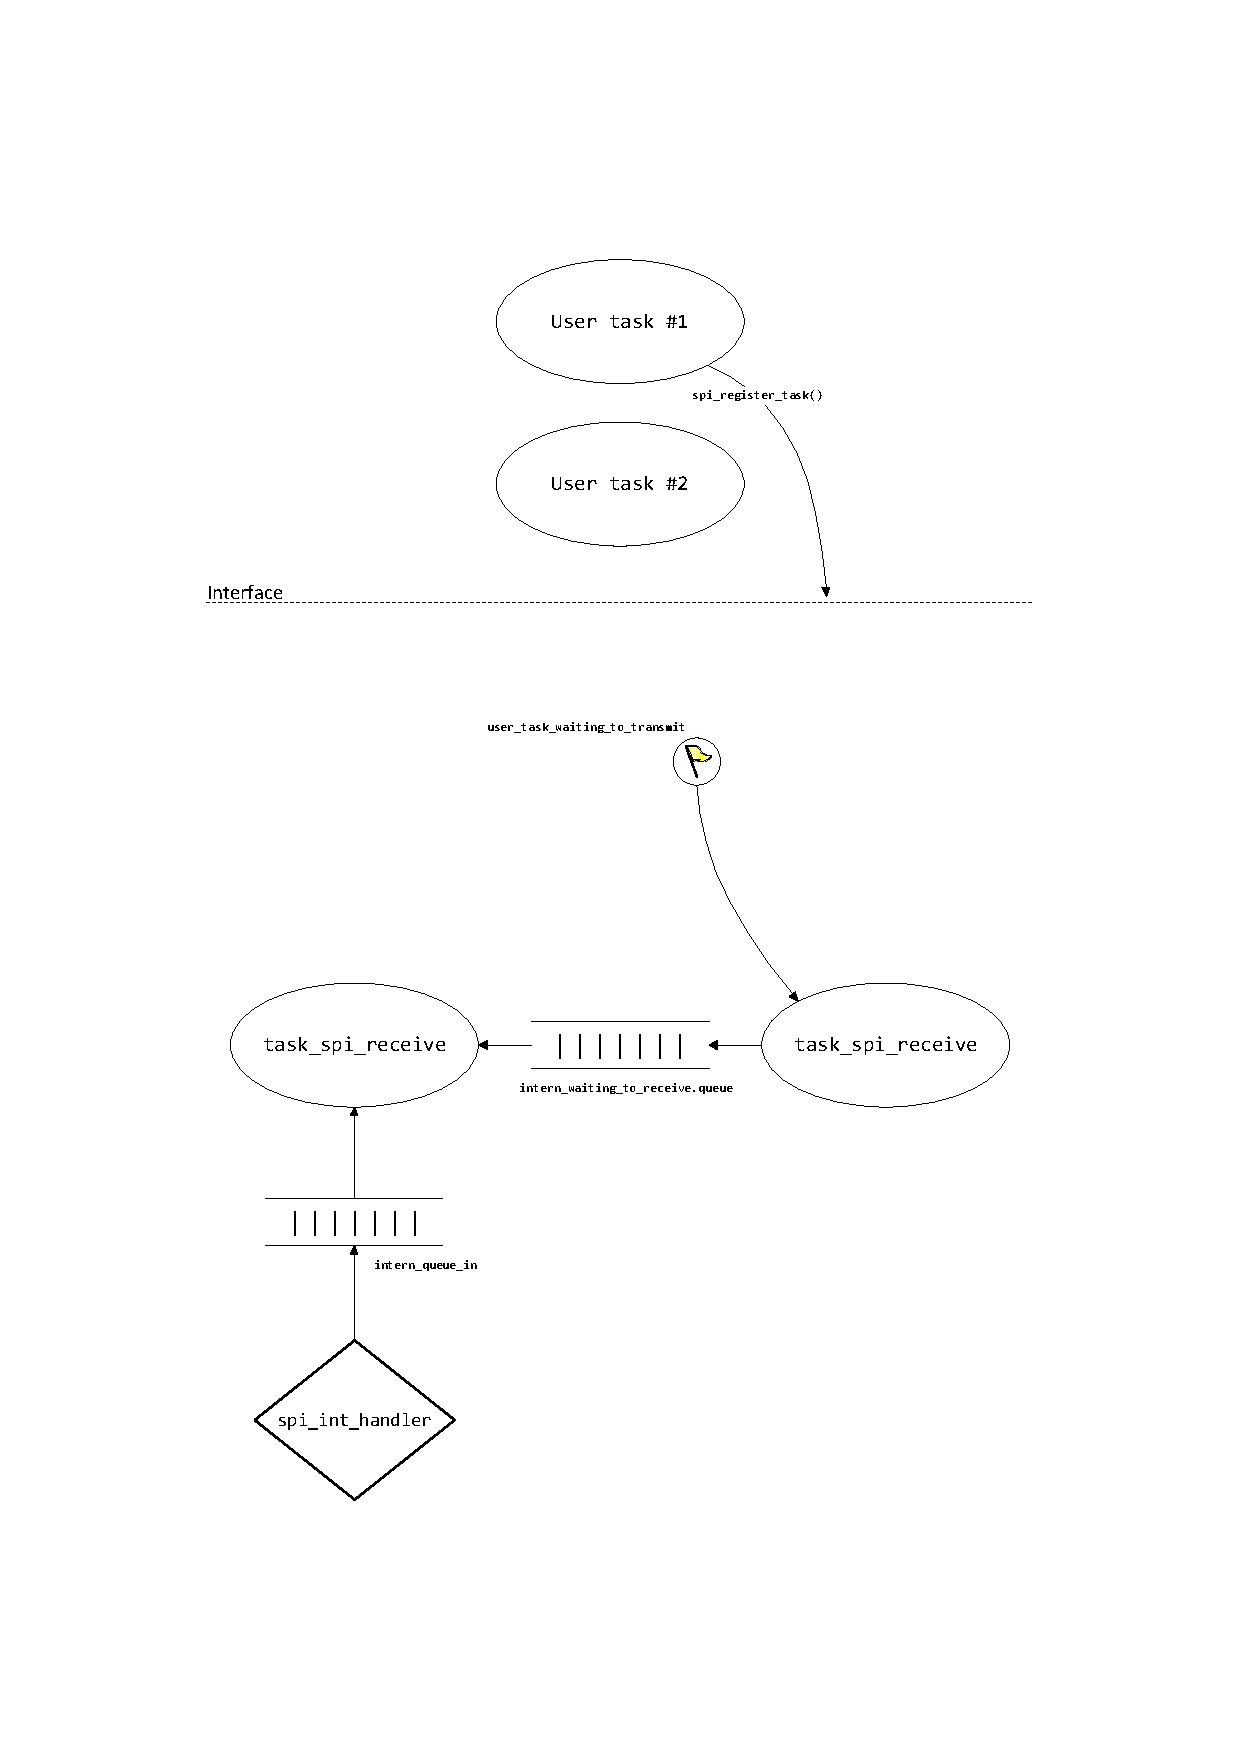
\includegraphics[width=\textwidth,clip,trim=12 -46 12 0]{content/04_communication/figures/spi_task_diagram_initial_1.pdf}
    \caption{Before the \texttt{spi\_register\_task} call.}
    \label{fig:spi_task_diagram_initial_1}
  \end{subfigure}
  \begin{subfigure}[b]{0.495\textwidth}
    \centering
    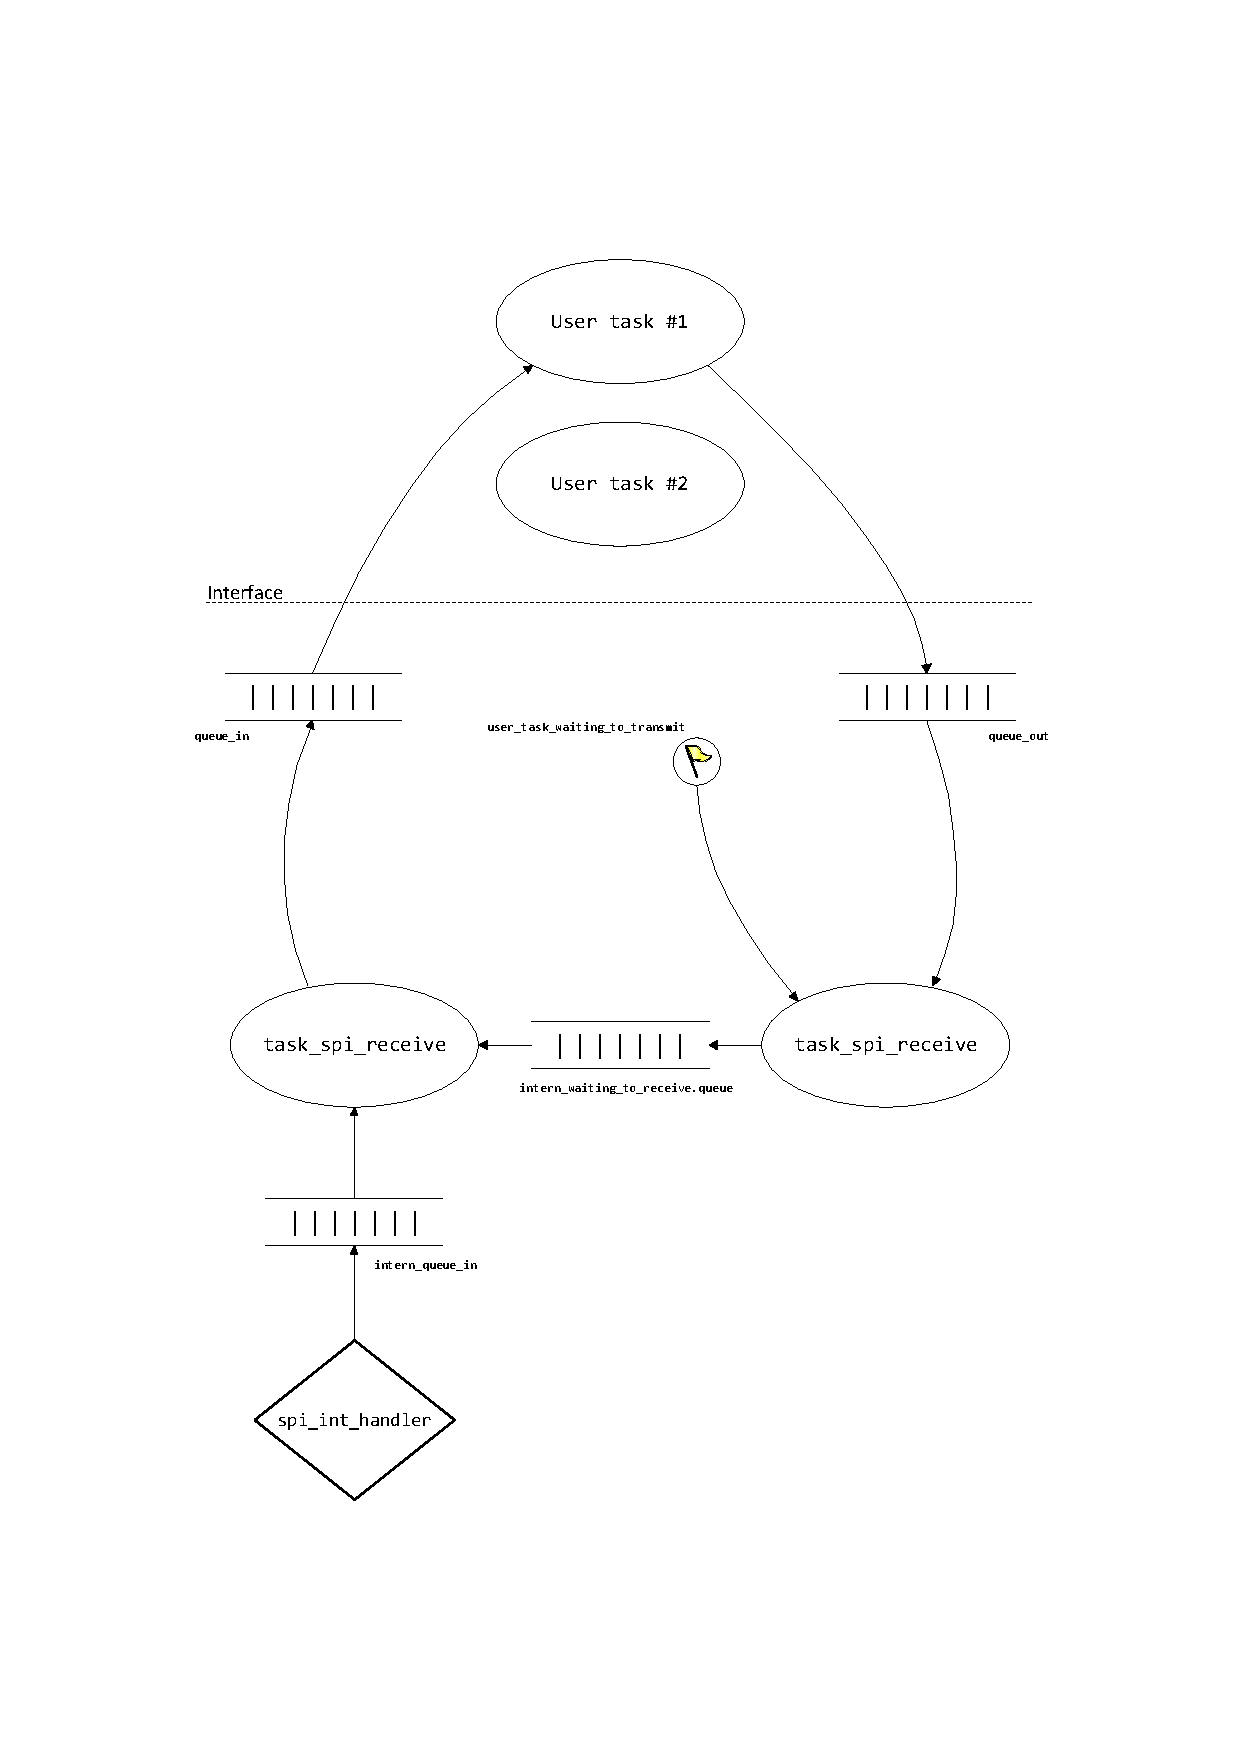
\includegraphics[width=\textwidth,clip,trim=12 0 12 0]{content/04_communication/figures/spi_task_diagram_initial_2.pdf}
    \caption{After the \texttt{spi\_register\_task} call.}
    \label{fig:spi_task_diagram_initial_2}
  \end{subfigure}
  \caption{A user task registering with the SPI interface.}
  \label{fig:spi_register_task}
\end{figure}%trim=l b r t

For a task to be able to use the SPI link, it will have to first make a call to the function \texttt{spi\_register\_task}. That is because resources are allocated dynamically, described in section \ref{sec:spi_underthehood}. Figure \ref{fig:spi_register_task} shows a user task using the register function and getting queues allocated to it. 

When a user task has been successfully registered with the SPI software it is allowed use of the \texttt{spi\_write\_from\_task}- and \texttt{spi\_read\_from\_task}-functions to read and write to and from its private queues. With only those two functions used frequently during runtime, the second design goal is considered fulfilled.

An overview - a task diagram - is shown in figure \ref{fig:spi_task_diagram}.



\subsection{Under the hood}\label{sec:spi_underthehood}
To understand how the implementation works, a description of what goes on ``under the hood'' follows. That is, between the user interface and the hardware transmit/receive logic. The first design goal was, that the implementation should be thread-safe. To elaborate; the implementation should allow multiple tasks to send and receive data asynchronously. To make that possible, a scheme, where each task gets its own private software buffers for transmission and reception, is used. That way the software implementation can imitate multiple SPI hardware interfaces. The implementation works is such a way that these ``private'' queues are allocated dynamically when a task wishes to use the SPI. The task which wishes to use the SPI is then associated with the queues by task handle.\footnote{A way of uniquely identifying tasks provided by the FreeRTOS API.} The private queues can be seen just below the ``interface line'' on the task diagram in figure \ref{fig:spi_task_diagram}.

\begin{figure}[htb]
  \centering
  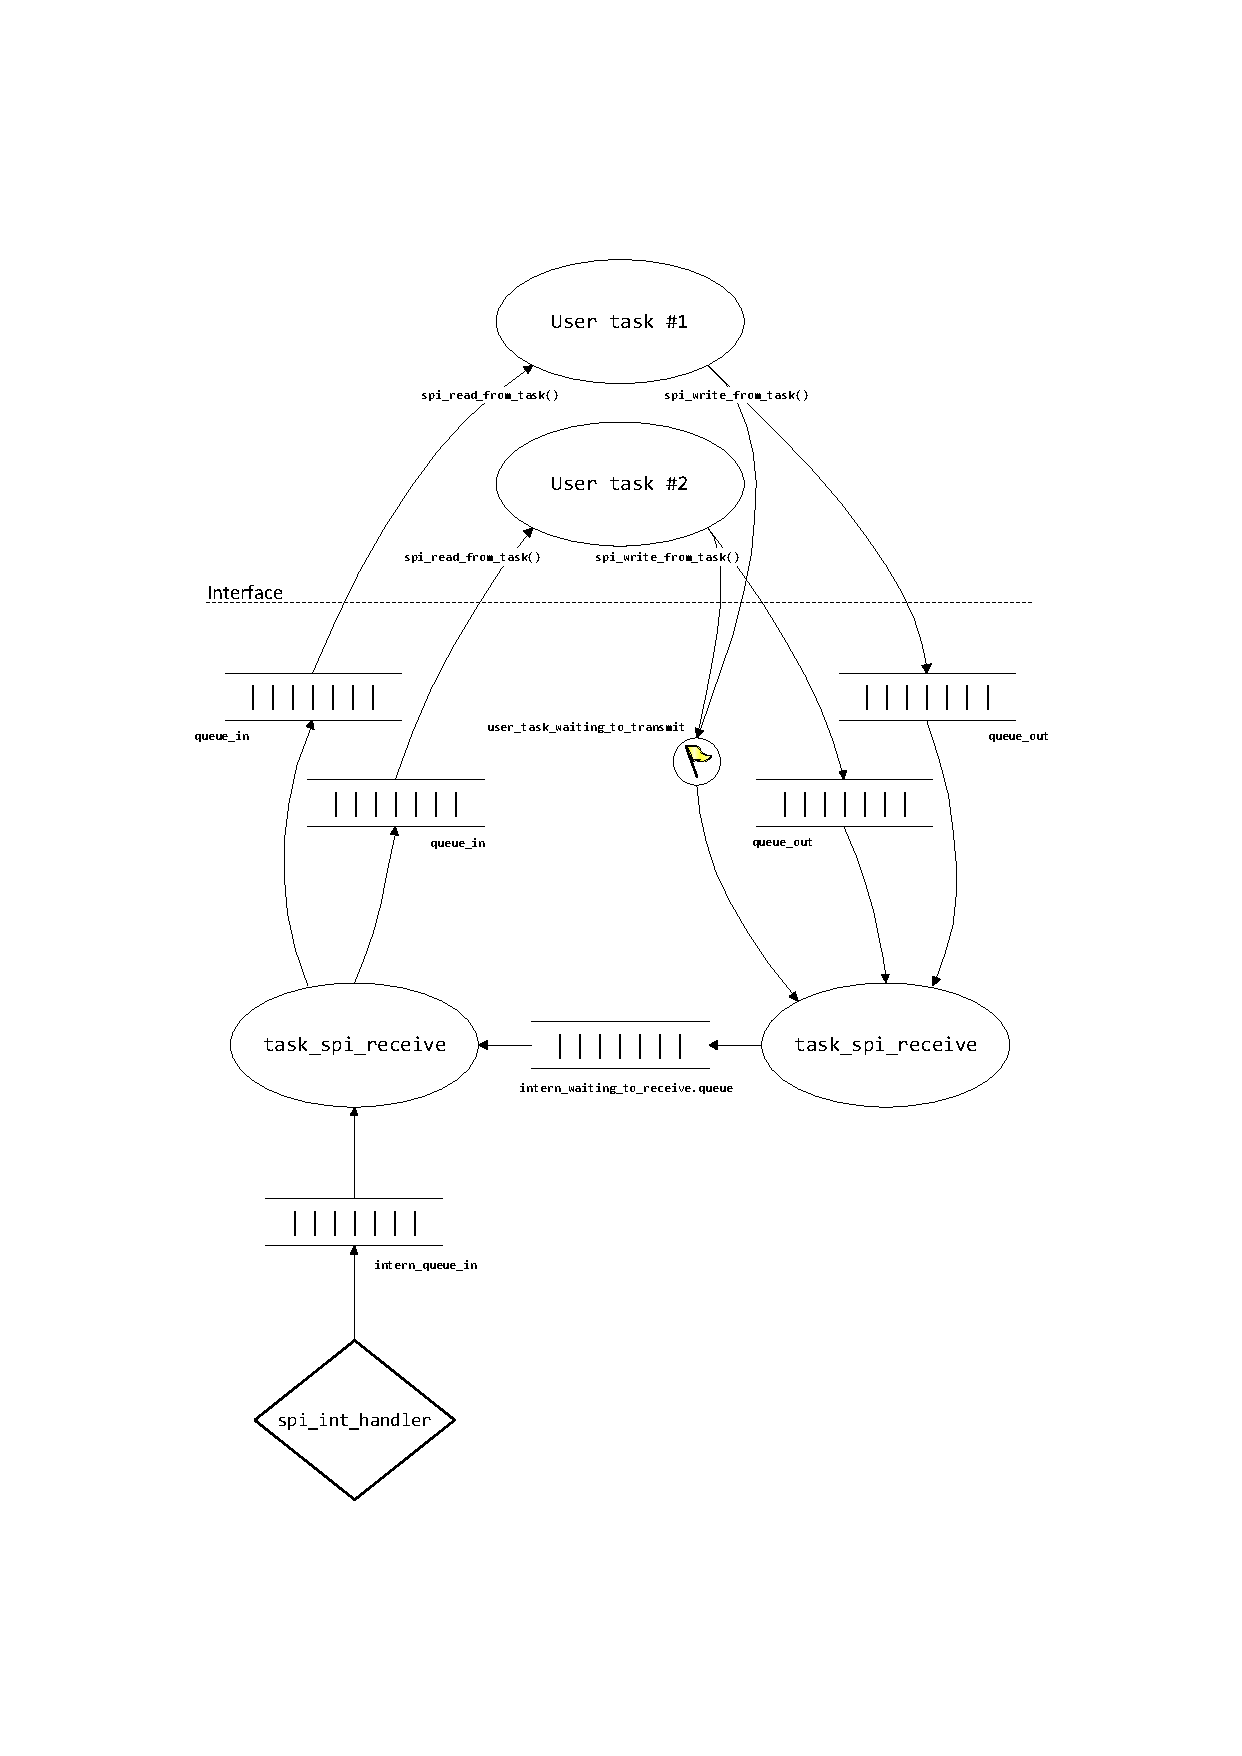
\includegraphics[width=0.94\textwidth,clip,trim=0 15 0 15]{content/04_communication/figures/spi_task_diagram_running.pdf}
  \caption{An overview of the SPI software implementation during normal operation.}
  \label{fig:spi_task_diagram}
\end{figure}%trim=l b r t

A doubly linked list is used to keep track of tasks using the SPI implementation. Each element in the list is a variable that contain the handle of the user task, associated queues and how many units of data they are waiting to receive. The linked list is semaphore-protected.

Two tasks are used to provide the transmit and receive functionality required: One for transmission and one for reception. Once a user task places data in its private transmission-queue, it is out of the user tasks hands: It can only wait for data to be received, so it can be read through \texttt{spi\_read\_from\_task}. It is the transmit task's responsibility to make sure the data items get sent, and it is the receiver task's responsibility to direct incoming data to the appropriate tasks reception queue.

Suppose a user task has placed a unit of data in its transmission-queue. At the same time, it must ``give''\footnote{Using FreeRTOS terminology, the functions to unlock resources protected by semaphores are all called \texttt{*SemaphoreGive*}} the binary semaphore \texttt{user\_task\_waiting\_to\_transmit}, which, when given, will un-block the transmit task. This is to avoid having the transmit task spending all of its scheduled time polling the user task transmit queues. When the transmit task is no longer blocked by the \texttt{user\_task\_waiting\_to\_transmit} semaphore, the kernel runs it soon after. When the task runs, it finds a user-task queue which contains items to send and places those items in the hardware transmit FIFO. At the same time, it saves the number of items sent in the variable contained in the linked list. The order in which different user tasks transmit and receive is kept track of by placing them in the queue \texttt{intern\_waiting\_to\_receive.queue} as shown in figure \ref{fig:spi_task_diagram}.

The receiver task blocks on incoming data which is provided by \texttt{spi\_int\_handler} ISR. When it receives a unit of data, it will look in the \texttt{intern\_waiting\_to\_receive.queue} to determine what task the incoming data is for. The data is then placed in that particular user-tasks receive-queue, which the user-task can read at will. It must be read frequently enough to keep up with the speed at which it the user task transmits, though.

\nomenclature{ISR}{Interrupt Service Routine}
